\documentclass[10pt]{article}
\usepackage[polish]{babel}
\usepackage[utf8]{inputenc}
\usepackage[T1]{fontenc}
\usepackage{amsmath}
\usepackage{amsfonts}
\usepackage{amssymb}
\usepackage[version=4]{mhchem}
\usepackage{stmaryrd}
\usepackage{graphicx}
\usepackage[export]{adjustbox}
\graphicspath{ {./images/} }

\title{ARKUSZ PRÓBNEJ MATURY Z OPERONEM MATEMATYKA }

\author{}
\date{}


\begin{document}
\maketitle
\section*{POZIOM PODSTAWOWY}
\section*{Czas pracy: \(\mathbf{1 7 0}\) minut}
\section*{Instrukcja dla zdającego}
\begin{enumerate}
  \item Sprawdź, czy arkusz egzaminacyjny zawiera 16 stron (zadania 1.-33.). Ewentualny brak zgłoś przewodniczącemu zespołu nadzorującego egzamin.
  \item Rozwiązania zadań i odpowiedzi zapisz w miejscu na to przeznaczonym.
  \item W zadaniach zamkniętych (1.-24.) zaznacz poprawną odpowiedź.
  \item W rozwiązaniach zadań otwartych (25.-33.) przedstaw tok rozumowania prowadzący do ostatecznego wyniku.
  \item Pisz czytelnie. Używaj długopisu/pióra tylko z czarnym tuszem/atramentem.
  \item Nie używaj korektora, a błędne zapisy wyraźnie przekreśl.
  \item Zapisy w brudnopisie nie będą oceniane.
  \item Obok numeru każdego zadania podana jest maksymalna liczba punktów możliwych do uzyskania.
  \item Możesz korzystać z zestawu wzorów matematycznych, cyrkla i linijki oraz kalkulatora.
\end{enumerate}

\section*{Życzymy powodzenia!}
Za rozwiązanie wszystkich zadań można otrzymać łącznie 50 punktów.\\

\includegraphics[max width=\textwidth, center]{2024_11_21_769d5953f978b92e06f5g-01}

\section*{KOD ZDAJĄCEGO}
LISTOPAD\\
2013

PESEL ZDAJĄCEGO\\
Wpisuje zdający przed rozpoczęciem pracy\\

\includegraphics[max width=\textwidth, center]{2024_11_21_769d5953f978b92e06f5g-01(1)}

\section*{ZADANIA ZAMKNIĘTE}
\section*{W zadaniach od 1. do 24. wybierz i zaznacz jedną poprawną odpowiedź.}
\section*{Zadanie 1. (1 pkt)}
Suma liczby odwrotnej do liczby \(-4 \frac{3}{5} \mathrm{i}\) liczby przeciwnej do liczby \(\frac{18}{23}\) jest równa:\\
A. -1\\
B. 0\\
C. \(-\frac{21}{23}\)\\
D. 1

\section*{Zadanie 2. (1 pkt)}
Wartość wyrażenia \(\frac{1}{2} \log _{3} 15-\log _{3} \sqrt{5}\) jest równa:\\
A. -1\\
B. \(\log _{3} 3 \sqrt{5}\)\\
C. \(\frac{1}{2}\)\\
D. 1

\section*{Zadanie 3. (1 pkt)}
Suma przedziałów \((-\infty,-11) \cup(7,+\infty)\) jest zbiorem rozwiązań nierówności:\\
A. \(|x+1|>10\)\\
B. \(|x+2|>9\)\\
C. \(|x-2|>11\)\\
D. \(|x+1|<10\)

\section*{Zadanie 4. (1 pkt)}
Niech \(k=2-3 \sqrt{2}\), zaś \(m=1-\sqrt{2}\). Wówczas wartość wyrażenia \(k^{2}-12 m\) jest równa:\\
A. \(21+12 \sqrt{2}\)\\
B. \(21-12 \sqrt{2}\)\\
C. 10\\
D. 34

\section*{Zadanie 5. (1 pkt)}
Liczba \(a\) stanowi \(40 \%\) liczby \(b\). Wówczas:\\
A. \(b=0,4 a\)\\
B. \(b=0,6 a\)\\
C. \(b=2,5 a\)\\
D. \(b=0,25 a\)

\section*{Zadanie 6. (1 pkt)}
Dziedziną funkcji \(f(x)=\frac{x+3}{x^{3}+4 x}\) jest zbiór:\\
A. \(R \backslash\{-4,0\}\)\\
B. \(R \backslash\{0\}\)\\
C. \(R\)\\
D. \(R \backslash\{-2,0,2\}\)

\section*{Zadanie 7. (1 pkt)}
Proste o równaniach \(-3 y-m x+12=0\) oraz \(y=6 x-12\) są prostopadłe dla \(m\) równego:\\
A. \(\frac{1}{2}\)\\
B. -18\\
C. \(-\frac{1}{2}\)\\
D. 6

\section*{BRUDNOPIS (nie podlega ocenie)}
\begin{center}

\includegraphics[max width=\textwidth]{2024_11_21_769d5953f978b92e06f5g-03}
\end{center}

\section*{Zadanie 8. (1 pkt)}
Zbiorem wartości funkcji \(f(x)=-2(x+3)(x-4)\) jest przedział:\\
A. \(\left(-\infty, 24 \frac{1}{2}\right)\)\\
B. \(\left\langle-24 \frac{1}{2},+\infty\right)\)\\
C. \(\left(24 \frac{1}{2},+\infty\right)\)\\
D. \(\left\langle-25 \frac{1}{2},+\infty\right)\)

\section*{Zadanie 9. (1 pkt)}
Na wykresie przedstawiony jest trójmian \(y=a x^{2}+b x+c\).\\
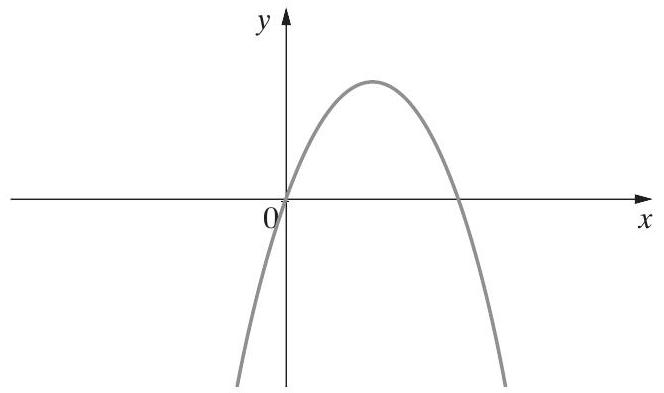
\includegraphics[max width=\textwidth, center]{2024_11_21_769d5953f978b92e06f5g-04}

Wynika z tego, że:\\
A. \(b<0\)\\
B. \(b>0\)\\
C. \(b \leq 0\)\\
D. \(b \geq 0\)

\section*{Zadanie 10. (1 pkt)}
Wielomian \(W(x)\) jest stopnia czwartego. Pierwiastkiem dwukrotnym tego wielomianu jest liczba -1 . Po rozłożeniu na czynniki wielomian ten może być postaci:\\
A. \(-2(x-1)^{2}\left(x^{2}+1\right)\)\\
B. \((x+1)^{2}(x-4)\)\\
C. \(-(x+1)^{2}\left(x^{2}+3\right)\)\\
D. \((x-1)(x+1)(x+2)(x-3)\)

\section*{Zadanie 11. (1 pkt)}
Liczba różnych rozwiązań równania \(\frac{(x+3)\left(x^{2}-4\right)}{x^{2}+2 x}=0\) wynosi:\\
A. 5\\
B. 4\\
C. 3\\
D. 2

\section*{Zadanie 12. (1 pkt)}
Dana jest funkcja \(h(x)=\left(-\frac{1}{3} m+2\right) x+\frac{3}{2} m-1\). Funkcja ta dla argumentu 0 przyjmuje war-\\
tość 5 . Wówczas:\\
A. \(m=9\)\\
B. \(m=6\)\\
C. \(m=4\)\\
D. \(m=2\)

\section*{Zadanie 13. (1 pkt)}
Ciąg \(\left(b_{n}\right)\) określony jest wzorem \(b_{n}=(-1)^{2 n+3}(n+1)\). Suma dwóch pierwszych wyrazów tego ciągu jest równa:\\
A. -5\\
B. -1\\
C. 1\\
D. 5

\section*{BRUDNOPIS (nie podlega ocenie)}
\begin{center}

\includegraphics[max width=\textwidth]{2024_11_21_769d5953f978b92e06f5g-05}
\end{center}

\section*{Zadanie 14. (1 pkt)}
W ciągu arytmetycznym piąty wyraz jest równy 8 , zaś siódmy wyraz tego ciągu jest równy 14. Dziesiąty wyraz tego ciągu jest równy:\\
A. 21\\
B. 23\\
C. 24\\
D. 3

\section*{Zadanie 15. (1 pkt)}
Pan Nowak wpłacił do banku \(k \mathrm{zł}\) na procent składany. Oprocentowanie w tym banku wynosi \(4 \%\) w skali roku, a odsetki kapitalizuje się co pół roku. Po 6 latach oszczędzania Pan Nowak zgromadzi na koncie kwotę:\\
A. \(k(1+0,02)^{12} \mathrm{zł}\)\\
B. \(k(1+0,04)^{12} \mathrm{zf}\)\\
C. \(k(1+0,02)^{6} \mathrm{zf}\)\\
D. \(k(1+0,4)^{6} \mathrm{zl}\)

\section*{Zadanie 16. (1 pkt)}
W trójkącie równoramiennym \(A B C\) (rys.) o wysokościach \(C D\) i \(A E\) podstawa \(A B\) ma długość 8 cm , a odcinek \(B E\) ma długość 3 cm . Długość odcinka \(A C\) jest równa:\\
A. 6 cm\\
B. \(\frac{32}{3} \mathrm{~cm}\)\\
C. \(\frac{28}{3} \mathrm{~cm}\)\\
D. \(\frac{33}{2} \mathrm{~cm}\)\\
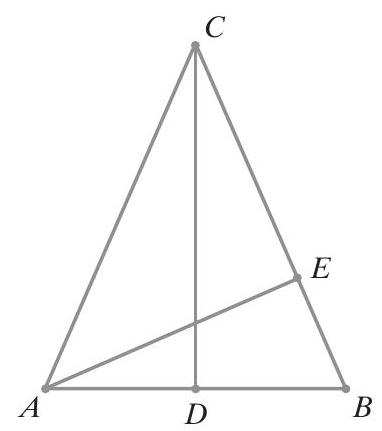
\includegraphics[max width=\textwidth, center]{2024_11_21_769d5953f978b92e06f5g-06}

\section*{Zadanie 17. (1 pkt)}
W czworokącie \(O B M A\) kąty wewnętrzne \(A O B\) i \(A M B\) mają równe miary (rys.).\\
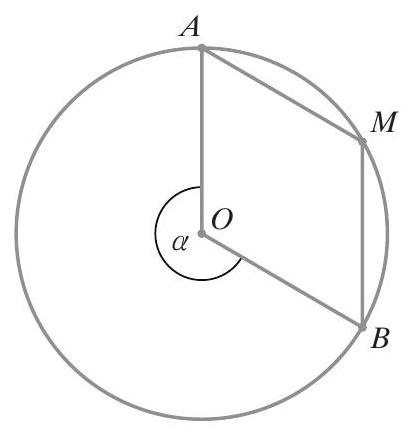
\includegraphics[max width=\textwidth, center]{2024_11_21_769d5953f978b92e06f5g-06(1)}

Wówczas kąt \(\alpha\) ma miarę:\\
A. \(160^{\circ}\)\\
B. \(120^{\circ}\)\\
C. \(240^{\circ}\)\\
D. \(210^{\circ}\)

\section*{Zadanie 18. (1 pkt)}
W trójkącie prostokątnym długość jednej z przyprostokątnych jest równa 7, zaś długość przeciwprostokątnej jest równa 8 . Zatem tangens mniejszego kąta ostrego w tym trójkącie jest równy:\\
A. \(\frac{15}{7}\)\\
B. \(\frac{8}{15}\)\\
C. \(\frac{\sqrt{15}}{7}\)\\
D. \(\frac{7 \sqrt{15}}{15}\)

\section*{BRUDNOPIS (nie podlega ocenie)}
\begin{center}

\includegraphics[max width=\textwidth]{2024_11_21_769d5953f978b92e06f5g-07}
\end{center}

\section*{Zadanie 19. (1 pkt)}
Długość odcinka \(B D\) w trójkącie prostokątnym \(A B C\) (rys.) jest równa:\\
A. \(\frac{9 \sqrt{3}}{4}\)\\
B. 4\\
C. \(4 \sqrt{3}\)\\
D. \(4 \sqrt{2}\)\\
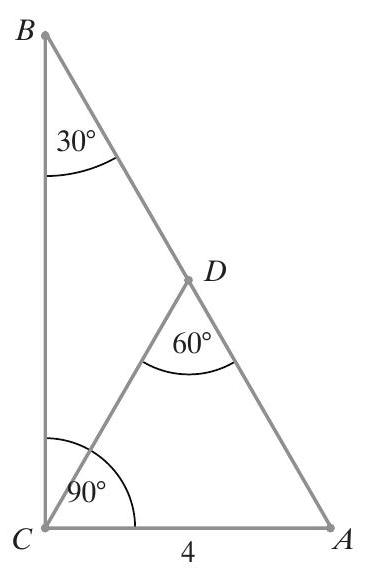
\includegraphics[max width=\textwidth, center]{2024_11_21_769d5953f978b92e06f5g-08}

\section*{Zadanie 20. (1 pkt)}
Pole koła wpisanego w trójkąt równoboczny jest równe \(\frac{16}{3} \pi\). Obwód tego trójkąta jest równy:\\
A. \(12 \sqrt{3}\)\\
B. 24\\
C. 12\\
D. 36

\section*{Zadanie 21. (1 pkt)}
Długość okręgu opisanego równaniem \(x^{2}-4 x+y^{2}-4=0\) jest równa:\\
A. \(4 \sqrt{2} \pi\)\\
B. \(4 \pi\)\\
C. \(2 \sqrt{2} \pi\)\\
D. \(8 \sqrt{2} \pi\)

\section*{Zadanie 22. (1 pkt)}
Punkty \(A=(-2,4)\) i \(C=(-6,2)\) są przeciwległymi wierzchołkami kwadratu \(A B C D\). Zatem promień okręgu opisanego na tym kwadracie jest równy:\\
A. 10\\
B. 2\\
C. \(\sqrt{5}\)\\
D. \(\sqrt{10}\)

\section*{Zadanie 23. (1 pkt)}
Ze zbioru liczb \(\{1,2,3,4,6,8,12,14,15\}\) wybieramy losowo jedną liczbę. Prawdopodobieństwo, że wybierzemy liczbę, której dzielnikiem jest liczba 3, wynosi:\\
A. \(\frac{5}{9}\)\\
B. \(\frac{4}{9}\)\\
C. \(\frac{1}{3}\)\\
D. \(\frac{2}{3}\)

\section*{Zadanie 24. (1 pkt)}
W ostrosłupie prawidłowym czworokątnym objętość jest równa 32, zaś krawędź podstawy jest równa 4. Wysokość tego ostrosłupa jest równa:\\
A. \(\frac{2}{3}\)\\
B. \(\frac{4}{3}\)\\
C. 2\\
D. 6

\section*{BRUDNOPIS (nie podlega ocenie)}
\begin{center}

\includegraphics[max width=\textwidth]{2024_11_21_769d5953f978b92e06f5g-09}
\end{center}

\section*{ZADANIA OTWARTE}
Rozwiązania zadań o numerach od 25. do 33. należy zapisać w wyznaczonych miejscach pod treścią zadania.

Zadanie 25. (2 pkt)\\
Rozwiąż nierówność: \(-2 x^{2}+3 x<4\).

\begin{center}
\begin{tabular}{|c|c|c|c|c|c|c|c|c|c|c|c|c|c|c|c|c|c|c|c|c|c|c|c|c|c|c|c|c|c|}
\hline
 &  &  &  &  &  &  &  &  &  &  &  &  &  &  &  &  &  &  &  &  &  &  &  &  &  &  &  &  &  \\
\hline
 &  &  &  &  &  &  &  &  &  &  &  &  &  &  &  &  &  &  &  &  &  &  &  &  &  &  &  &  &  \\
\hline
 &  &  &  &  &  &  &  &  &  &  &  &  &  &  &  &  &  &  &  &  &  &  &  &  &  &  &  &  &  \\
\hline
 &  &  &  &  &  &  &  &  &  &  &  &  &  &  &  &  &  &  &  &  &  &  &  &  &  &  &  &  &  \\
\hline
 &  &  &  &  &  &  &  &  &  &  &  &  &  &  &  &  &  &  &  &  &  &  &  &  &  &  &  &  &  \\
\hline
 &  &  &  &  &  &  &  &  &  &  &  &  &  &  &  &  &  &  &  &  &  &  &  &  &  &  &  &  &  \\
\hline
 &  &  &  &  &  &  &  &  &  &  &  &  &  &  &  &  &  &  &  &  &  &  &  &  &  &  &  &  &  \\
\hline
 &  &  &  &  &  &  &  &  &  &  &  &  &  &  &  &  &  &  &  &  &  &  &  &  &  &  &  &  &  \\
\hline
 &  &  &  &  &  &  &  &  &  &  &  &  &  &  &  &  &  &  &  &  &  &  &  &  &  &  &  &  &  \\
\hline
 &  &  &  &  &  &  &  &  &  &  &  &  &  &  &  &  &  &  &  &  &  &  &  &  &  &  &  &  &  \\
\hline
 &  &  &  &  &  &  &  &  &  &  &  &  &  &  &  &  &  &  &  &  &  &  &  &  &  &  &  &  &  \\
\hline
 &  &  &  &  &  &  &  &  &  &  &  &  &  &  &  &  &  &  &  &  &  &  &  &  &  &  &  &  &  \\
\hline
 &  &  &  &  &  &  &  &  &  &  &  &  &  &  &  &  &  &  &  &  &  &  &  &  &  &  &  &  &  \\
\hline
 &  &  &  &  &  &  &  &  &  &  &  &  &  &  &  &  &  &  &  &  &  &  &  &  &  &  &  &  &  \\
\hline
\end{tabular}
\end{center}

Odpowiedź:

\section*{Zadanie 26. (2 pkt)}
Dany jest wielomian \(W(x)=-2 x^{3}+3 x^{2}-(k+2) x-6\). Wyznacz wartość \(k\), wiedząc, że liczba -2 jest pierwiastkiem wielomianu \(W(x)\).\\

\includegraphics[max width=\textwidth, center]{2024_11_21_769d5953f978b92e06f5g-10}

Odpowiedź:

\section*{Zadanie 27. (2 pkt)}
Wykaż, że trapez, w którym przekątne dzielą kąty przy dłuższej podstawie na połowy, jest równoramienny.

\begin{center}
\begin{tabular}{|c|c|c|c|c|c|c|c|c|c|c|c|c|c|c|c|c|c|c|c|c|c|c|}
\hline
 &  &  &  &  &  &  &  &  &  &  &  &  &  &  &  &  &  &  &  &  &  &  \\
\hline
 &  &  &  &  &  &  &  &  &  &  &  &  &  &  &  &  &  &  &  &  &  &  \\
\hline
 &  &  &  &  &  &  &  &  &  &  &  &  &  &  &  &  &  &  &  &  &  &  \\
\hline
 &  &  &  &  &  &  &  &  &  &  &  &  &  &  &  &  &  &  &  &  &  &  \\
\hline
 &  &  &  &  &  &  &  &  &  &  &  &  &  &  &  &  &  &  &  &  &  &  \\
\hline
 &  &  &  &  &  &  &  &  &  &  &  &  &  &  &  &  &  &  &  &  &  &  \\
\hline
 &  &  &  &  &  &  &  &  &  &  &  &  &  &  &  &  &  &  &  &  &  &  \\
\hline
 &  &  &  &  &  &  &  &  &  &  &  &  &  &  &  &  &  &  &  &  &  &  \\
\hline
 &  &  &  &  &  &  &  &  &  &  &  &  &  &  &  &  &  &  &  &  &  &  \\
\hline
 &  &  &  &  &  &  &  &  &  &  &  &  &  &  &  &  &  &  &  &  &  &  \\
\hline
 &  &  &  &  &  &  &  &  &  &  &  &  &  &  &  &  &  &  &  &  &  &  \\
\hline
 &  &  &  &  &  &  &  &  &  &  &  &  &  &  &  &  &  &  &  &  &  &  \\
\hline
 &  &  &  &  &  &  &  &  &  &  &  &  &  &  &  &  &  &  &  &  &  &  \\
\hline
 &  &  &  &  &  &  &  &  &  &  &  &  &  &  &  &  &  &  &  &  &  &  \\
\hline
 &  &  &  &  &  &  &  &  &  &  &  &  &  &  &  &  &  &  &  &  &  &  \\
\hline
 &  &  &  &  &  &  &  &  &  &  &  &  &  &  &  &  &  &  &  &  &  &  \\
\hline
 &  &  &  &  &  &  &  &  &  &  &  &  &  &  &  &  &  &  &  &  &  &  \\
\hline
\end{tabular}
\end{center}

Odpowiedź: \(\qquad\)

\section*{Zadanie 28. (2 pkt)}
Maszt telekomunikacyjny rzuca cień, który jest 2 razy krótszy niż wysokość masztu. Oblicz cosinus kąta, pod jakim padają promienie słoneczne.

\begin{center}
\begin{tabular}{|c|c|c|c|c|c|c|c|c|c|c|c|c|c|c|c|c|c|c|c|c|c|c|c|}
\hline
 &  &  &  &  &  &  &  &  &  &  &  &  &  &  &  &  &  &  &  &  &  &  &  \\
\hline
 &  &  &  &  &  &  &  &  &  &  &  &  &  &  &  &  &  &  &  &  &  &  &  \\
\hline
 &  &  &  &  &  &  &  &  &  &  &  &  &  &  &  &  &  &  &  &  &  &  &  \\
\hline
 &  &  &  &  &  &  &  &  &  &  &  &  &  &  &  &  &  &  &  &  &  &  &  \\
\hline
 &  &  &  &  &  &  &  &  &  &  &  &  &  &  &  &  &  &  &  &  &  &  &  \\
\hline
 &  &  &  &  &  &  &  &  &  &  &  &  &  &  &  &  &  &  &  &  &  &  &  \\
\hline
 &  &  &  &  &  &  &  &  &  &  &  &  &  &  &  &  &  &  &  &  &  &  &  \\
\hline
 &  &  &  &  &  &  &  &  &  &  &  &  &  &  &  &  &  &  &  &  &  &  &  \\
\hline
 &  &  &  &  &  &  &  &  &  &  &  &  &  &  &  &  &  &  &  &  &  &  &  \\
\hline
 &  &  &  &  &  &  &  &  &  &  &  &  &  &  &  &  &  &  &  &  &  &  &  \\
\hline
 &  &  &  &  &  &  &  &  &  &  &  &  &  &  &  &  &  &  &  &  &  &  &  \\
\hline
 &  &  &  &  &  &  &  &  &  &  &  &  &  &  &  &  &  &  &  &  &  &  &  \\
\hline
 &  &  &  &  &  &  &  &  &  &  &  &  &  &  &  &  &  &  &  &  &  &  &  \\
\hline
 &  &  &  &  &  &  &  &  &  &  &  &  &  &  &  &  &  &  &  &  &  &  &  \\
\hline
 &  &  &  &  &  &  &  &  &  &  &  &  &  &  &  &  &  &  &  &  &  &  &  \\
\hline
 &  &  &  &  &  &  &  &  &  &  &  &  &  &  &  &  &  &  &  &  &  &  &  \\
\hline
 &  &  &  &  &  &  &  &  &  &  &  &  &  &  &  &  &  &  &  &  &  &  &  \\
\hline
\end{tabular}
\end{center}

Odpowiedź: \(\qquad\)

\section*{Zadanie 29. (2 pkt)}
Dwa okręgi są styczne zewnętrznie. Odległość ich środków jest równa 8 cm . Gdyby te okręgi były styczne wewnętrznie, to odległość ich środków byłaby równa 2 cm . Oblicz długości promieni tych okręgów.

\begin{center}
\begin{tabular}{|c|c|c|c|c|c|c|c|c|c|c|c|c|c|c|c|c|c|c|c|c|c|c|c|c|c|c|c|c|c|}
\hline
 &  &  &  &  &  &  &  &  &  &  &  &  &  &  &  &  &  &  &  &  &  &  &  &  &  &  &  &  &  \\
\hline
 &  &  &  &  &  &  &  &  &  &  &  &  &  &  &  &  &  &  &  &  &  &  &  &  &  &  &  &  &  \\
\hline
 &  &  &  &  &  &  &  &  &  &  &  &  &  &  &  &  &  &  &  &  &  &  &  &  &  &  &  &  &  \\
\hline
 &  &  &  &  &  &  &  &  &  &  &  &  &  &  &  &  &  &  &  &  &  &  &  &  &  &  &  &  &  \\
\hline
 &  &  &  &  &  &  &  &  &  &  &  &  &  &  &  &  &  &  &  &  &  &  &  &  &  &  &  &  &  \\
\hline
 &  &  &  &  &  &  &  &  &  &  &  &  &  &  &  &  &  &  &  &  &  &  &  &  &  &  &  &  &  \\
\hline
 &  &  &  &  &  &  &  &  &  &  &  &  &  &  &  &  &  &  &  &  &  &  &  &  &  &  &  &  &  \\
\hline
 &  &  &  &  &  &  &  &  &  &  &  &  &  &  &  &  &  &  &  &  &  &  &  &  &  &  &  &  &  \\
\hline
 &  &  &  &  &  &  &  &  &  &  &  &  &  &  &  &  &  &  &  &  &  &  &  &  &  &  &  &  &  \\
\hline
 &  &  &  &  &  &  &  &  &  &  &  &  &  &  &  &  &  &  &  &  &  &  &  &  &  &  &  &  &  \\
\hline
 &  &  &  &  &  &  &  &  &  &  &  &  &  &  &  &  &  &  &  &  &  &  &  &  &  &  &  &  &  \\
\hline
 &  &  &  &  &  &  &  &  &  &  &  &  &  &  &  &  &  &  &  &  &  &  &  &  &  &  &  &  &  \\
\hline
 &  &  &  &  &  &  &  &  &  &  &  &  &  &  &  &  &  &  &  &  &  &  &  &  &  &  &  &  &  \\
\hline
 &  &  &  &  &  &  &  &  &  &  &  &  &  &  &  &  &  &  &  &  &  &  &  &  &  &  &  &  &  \\
\hline
 &  &  &  &  &  &  &  &  &  &  &  &  &  &  &  &  &  &  &  &  &  &  &  &  &  &  &  &  &  \\
\hline
 &  &  &  &  &  &  &  &  &  &  &  &  &  &  &  &  &  &  &  &  &  &  &  &  &  &  &  &  &  \\
\hline
 &  &  &  &  &  &  &  &  &  &  &  &  &  &  &  &  &  &  &  &  &  &  &  &  &  &  &  &  &  \\
\hline
\end{tabular}
\end{center}

Odpowiedź:

\section*{Zadanie 30. (2 pkt)}
Dany jest trójkąt \(A B C\), gdzie \(A=(-3,-2), B=(1,-1), C=(-1,4)\). Wyznacz równanie symetralnej boku \(A C\) tego trójkąta.\\

\includegraphics[max width=\textwidth, center]{2024_11_21_769d5953f978b92e06f5g-12}

Odpowiedź:

\section*{Zadanie 31. (4 pkt)}
Uczeń przygotowujący się do matury w ciągu pierwszego tygodnia rozwiązał 5 zadań. Postanowił jednak, że w każdym następnym tygodniu będzie rozwiązywał o 2 zadania więcej niż w poprzednim tygodniu. W którym tygodniu liczba zadań rozwiązanych przez niego od początku nauki przekroczy 480?

\begin{center}
\begin{tabular}{|c|c|c|c|c|c|c|c|c|c|c|c|c|c|c|c|c|c|c|c|c|}
\hline
 &  &  &  &  &  &  &  &  &  &  &  &  &  &  &  &  &  &  &  &  \\
\hline
 &  &  &  &  &  &  &  &  &  &  &  &  &  &  &  &  &  &  &  &  \\
\hline
 &  &  &  &  &  &  &  &  &  &  &  &  &  &  &  &  &  &  &  &  \\
\hline
 &  &  &  &  &  &  &  &  &  &  &  &  &  &  &  &  &  &  &  &  \\
\hline
 &  &  &  &  &  &  &  &  &  &  &  &  &  &  &  &  &  &  &  &  \\
\hline
 &  &  &  &  &  &  &  &  &  &  &  &  &  &  &  &  &  &  &  &  \\
\hline
 &  &  &  &  &  &  &  &  &  &  &  &  &  &  &  &  &  &  &  &  \\
\hline
 &  &  &  &  &  &  &  &  &  &  &  &  &  &  &  &  &  &  &  &  \\
\hline
 &  &  &  &  &  &  &  &  &  &  &  &  &  &  &  &  &  &  &  &  \\
\hline
 &  &  &  &  &  &  &  &  &  &  &  &  &  &  &  &  &  &  &  &  \\
\hline
 &  &  &  &  &  &  &  &  &  &  &  &  &  &  &  &  &  &  &  &  \\
\hline
 &  &  &  &  &  &  &  &  &  &  &  &  &  &  &  &  &  &  &  &  \\
\hline
 &  &  &  &  &  &  &  &  &  &  &  &  &  &  &  &  &  &  &  &  \\
\hline
 &  &  &  &  &  &  &  &  &  &  &  &  &  &  &  &  &  &  &  &  \\
\hline
 &  &  &  &  &  &  &  &  &  &  &  &  &  &  &  &  &  &  &  &  \\
\hline
 &  &  &  &  &  &  &  &  &  &  &  &  &  &  &  &  &  &  &  &  \\
\hline
 &  &  &  &  &  &  &  &  &  &  &  &  &  &  &  &  &  &  &  &  \\
\hline
 &  &  &  &  &  &  &  &  &  &  &  &  &  &  &  &  &  &  &  &  \\
\hline
 &  &  &  &  &  &  &  &  &  &  &  &  &  &  &  &  &  &  &  &  \\
\hline
 &  &  &  &  &  &  &  &  &  &  &  &  &  &  &  &  &  &  &  &  \\
\hline
 &  &  &  &  &  &  &  &  &  &  &  &  &  &  &  &  &  &  &  &  \\
\hline
 &  &  &  &  &  &  &  &  &  &  &  &  &  &  &  &  &  &  &  &  \\
\hline
 &  &  &  &  &  &  &  &  &  &  &  &  &  &  &  &  &  &  &  &  \\
\hline
 &  &  &  &  &  &  &  &  &  &  &  &  &  &  &  &  &  &  &  &  \\
\hline
 &  &  &  &  &  &  &  &  &  &  &  &  &  &  &  &  &  &  &  &  \\
\hline
 &  &  &  &  &  &  &  &  &  &  &  &  &  &  &  &  &  &  &  &  \\
\hline
 &  &  &  &  &  &  &  &  &  &  &  &  &  &  &  &  &  &  &  &  \\
\hline
 &  &  &  &  &  &  &  &  &  &  &  &  &  &  &  &  &  &  &  &  \\
\hline
 &  &  &  &  &  &  &  &  &  &  &  &  &  &  &  &  &  &  &  &  \\
\hline
 &  &  &  &  &  &  &  &  &  &  &  &  &  &  &  &  &  &  &  &  \\
\hline
 &  &  &  &  &  &  &  &  &  &  &  &  &  &  &  &  &  &  &  &  \\
\hline
 &  &  &  &  &  &  &  &  &  &  &  &  &  &  &  &  &  &  &  &  \\
\hline
 &  &  &  &  &  &  &  &  &  &  &  &  &  &  &  &  &  &  &  &  \\
\hline
 &  &  &  &  &  &  &  &  &  &  &  &  &  &  &  &  &  &  &  &  \\
\hline
 &  &  &  &  &  &  &  &  &  &  &  &  &  &  &  &  &  &  &  &  \\
\hline
 &  &  &  &  &  &  &  &  &  &  &  &  &  &  &  &  &  &  &  &  \\
\hline
 &  &  &  &  &  &  &  &  &  &  &  &  &  &  &  &  &  &  &  &  \\
\hline
 &  &  &  &  &  &  &  &  &  &  &  &  &  &  &  &  &  &  &  &  \\
\hline
 &  &  &  &  &  &  &  &  &  &  &  &  &  &  &  &  &  &  &  &  \\
\hline
\end{tabular}
\end{center}

Odpowiedź:

\section*{Zadanie 32. (5 pkt)}
W graniastosłupie prawidłowym czworokątnym wysokość graniastosłupa jest o 4 krótsza od przekątnej podstawy i o 8 krótsza od przekątnej graniastosłupa. Oblicz sinus kąta pomiędzy przekątną graniastosłupa a płaszczyzną podstawy.\\

\includegraphics[max width=\textwidth, center]{2024_11_21_769d5953f978b92e06f5g-14}

Odpowiedź:

\section*{Zadanie 33. (5 pkt)}
Ojciec i syn zbierają w sadzie jabłka do skrzynek, które wkładają do samochodu dostawczego. Pracując jednocześnie, mogą załadować cały samochód w ciągu 6 godzin. Gdyby ojciec pracował sam, to załadowałby cały samochód w czasie o 5 godzin krótszym niż czas, w którym samodzielnie zrobiłby to syn. Oblicz, w jakim czasie ojciec załadowałby cały samochód, gdyby pracował sam.

\begin{center}
\begin{tabular}{|c|c|c|c|c|c|c|c|c|c|c|c|c|c|c|c|c|c|c|c|c|c|}
\hline
 &  &  &  &  &  &  &  &  &  &  &  &  &  &  &  &  &  &  &  &  &  \\
\hline
 &  &  &  &  &  &  &  &  &  &  &  &  &  &  &  &  &  &  &  &  &  \\
\hline
 &  &  &  &  &  &  &  &  &  &  &  &  &  &  &  &  &  &  &  &  &  \\
\hline
 &  &  &  &  &  &  &  &  &  &  &  &  &  &  &  &  &  &  &  &  &  \\
\hline
 &  &  &  &  &  &  &  &  &  &  &  &  &  &  &  &  &  &  &  &  &  \\
\hline
 &  &  &  &  &  &  &  &  &  &  &  &  &  &  &  &  &  &  &  &  &  \\
\hline
 &  &  &  &  &  &  &  &  &  &  &  &  &  &  &  &  &  &  &  &  &  \\
\hline
 &  &  &  &  &  &  &  &  &  &  &  &  &  &  &  &  &  &  &  &  &  \\
\hline
 &  &  &  &  &  &  &  &  &  &  &  &  &  &  &  &  &  &  &  &  &  \\
\hline
 &  &  &  &  &  &  &  &  &  &  &  &  &  &  &  &  &  &  &  &  &  \\
\hline
 &  &  &  &  &  &  &  &  &  &  &  &  &  &  &  &  &  &  &  &  &  \\
\hline
 &  &  &  &  &  &  &  &  &  &  &  &  &  &  &  &  &  &  &  &  &  \\
\hline
 &  &  &  &  &  &  &  &  &  &  &  &  &  &  &  &  &  &  &  &  &  \\
\hline
 &  &  &  &  &  &  &  &  &  &  &  &  &  &  &  &  &  &  &  &  &  \\
\hline
 &  &  &  &  &  &  &  &  &  &  &  &  &  &  &  &  &  &  &  &  &  \\
\hline
 &  &  &  &  &  &  &  &  &  &  &  &  &  &  &  &  &  &  &  &  &  \\
\hline
 &  &  &  &  &  &  &  &  &  &  &  &  &  &  &  &  &  &  &  &  &  \\
\hline
 &  &  &  &  &  &  &  &  &  &  &  &  &  &  &  &  &  &  &  &  &  \\
\hline
 &  &  &  &  &  &  &  &  &  &  &  &  &  &  &  &  &  &  &  &  &  \\
\hline
 &  &  &  &  &  &  &  &  &  &  &  &  &  &  &  &  &  &  &  &  &  \\
\hline
 &  &  &  &  &  &  &  &  &  &  &  &  &  &  &  &  &  &  &  &  &  \\
\hline
 &  &  &  &  &  &  &  &  &  &  &  &  &  &  &  &  &  &  &  &  &  \\
\hline
 &  &  &  &  &  &  &  &  &  &  &  &  &  &  &  &  &  &  &  &  &  \\
\hline
 &  &  &  &  &  &  &  &  &  &  &  &  &  &  &  &  &  &  &  &  &  \\
\hline
 &  &  &  &  &  &  &  &  &  &  &  &  &  &  &  &  &  &  &  &  &  \\
\hline
 &  &  &  &  &  &  &  &  &  &  &  &  &  &  &  &  &  &  &  &  &  \\
\hline
 &  &  &  &  &  &  &  &  &  &  &  &  &  &  &  &  &  &  &  &  &  \\
\hline
 &  &  &  &  &  &  &  &  &  &  &  &  &  &  &  &  &  &  &  &  &  \\
\hline
 &  &  &  &  &  &  &  &  &  &  &  &  &  &  &  &  &  &  &  &  &  \\
\hline
 &  &  &  &  &  &  &  &  &  &  &  &  &  &  &  &  &  &  &  &  &  \\
\hline
 &  &  &  &  &  &  &  &  &  &  &  &  &  &  &  &  &  &  &  &  &  \\
\hline
 &  &  &  &  &  &  &  &  &  &  &  &  &  &  &  &  &  &  &  &  &  \\
\hline
 &  &  &  &  &  &  &  &  &  &  &  &  &  &  &  &  &  &  &  &  &  \\
\hline
 &  &  &  &  &  &  &  &  &  &  &  &  &  &  &  &  &  &  &  &  &  \\
\hline
 &  &  &  &  &  &  &  &  &  &  &  &  &  &  &  &  &  &  &  &  &  \\
\hline
 &  &  &  &  &  &  &  &  &  &  &  &  &  &  &  &  &  &  &  &  &  \\
\hline
 &  &  &  &  &  &  &  &  &  &  &  &  &  &  &  &  &  &  &  &  &  \\
\hline
 &  &  &  &  &  &  &  &  &  &  &  &  &  &  &  &  &  &  &  &  &  \\
\hline
\end{tabular}
\end{center}

Odpowiedź:

\section*{BRUDNOPIS (nie podlega ocenie)}
\begin{center}

\includegraphics[max width=\textwidth]{2024_11_21_769d5953f978b92e06f5g-16}
\end{center}


\end{document}